\documentclass{swfcthesis}

\usepackage{todonotes}
\usepackage[inline]{enumitem}

\makeatletter
% This command ignores the optional argument for itemize and enumerate lists
\newcommand{\inlineitem}[1][]{%
\ifnum\enit@type=\tw@
    {\descriptionlabel{#1}}
  \hspace{\labelsep}%
\else
  \ifnum\enit@type=\z@
       \refstepcounter{\@listctr}\fi
    \quad\@itemlabel\hspace{\labelsep}%
\fi}
\makeatother
\parindent=0pt

\addbibresource{thesis.bib}    % 参照教程自己去写一个.bib文件

\begin{document}

\Title{RongOS --- 简单操作系统的实现}
\School{大数据与智能工程学院}
\Author{蒲启元}
\Advisor{王晓林}
\AdvisorTitle{讲师}
\AdvisorInfo{王晓林,男,49岁,硕士,讲师,毕业于英国格林尼治大学,分布式系统专业,现
  任西南林业大学计信学院教师,执教Linux、操作系统、网络技术等方面的课程,有丰富的Linux教学
  和系统管理经验。}
\Month{六}
\Year{二〇一八}

\Subject{计算机科学与技术专业} %专业名称(比如 电子信息工程专业)

\Abstract{操作系统管理着计算机的硬件和软件资源,它是向上层应用软件提供服务(接口)的核心系
  统软件,这些服务包括进程管理,内存管理,文件系统,网络通信,安全机制等。操作系统的设计与
  实现则是软件工业的基础。为此,在国务院提出的《中国制造2025》中专门强调了操作系统的开
  发\cite{china_2025}。但长期以来,操作系统核心开发技术都掌握在外国人手中,技术受制,对于我
  们的软件工业来说很不利。本项目从零开始设计开发个简单的操作系统,包括boot loader,中断,内
  存管理,图形接口,多任务,以及在这个系统上的几个小应用等。尽管这个系统很简单,但它为自主
  开发操作系统做了尝试。}

\Keywords{操作系统,进程,内存,中断,boot loader}

\Acknowledgments{首先我想感谢我的老师,王晓林。大学期间,他给了我很多指导,包括专业方面和上
  大学的意义等。很多时候,他对学生的要求看起来都是不近情理的,但正是通过这个“痛苦”的过程,
  我锻炼了坚强的意志,和战胜困难的信心。谢谢你,王老师。我最想感谢的是我的女友,她容忍我在
  完成这个设计时的很多个夜晚不陪她,给我支持,鼓励我,不抱怨。所以我愿意把这个简单操作系统
  命名为RongOS, 蓉便是她名字的最后一个字。谢谢你,我最亲爱的。}

\enTitle{RongOS --- A simple OS implementation}

\enAuthor{Qiyuan Pu}

\enAbstract{Operating system manages the resources of hardware and software, it lies
  in the core of the system software and provides services(interfaces) to upper
  applications. These services include process management, memory management, file system,
  network communication, security mechanism and more. Operating system development is the
  foundation and core of software industry. Therefore, \emph{Made in China
    2025} emphasizes the development of operating system that put forward by The State
  Council of China. For a long time, however, the OS kernel development technology is mastered
  by foreigner, due to technical limitations it is detrimental to our software industry. So this project will design and develop a simple operating system, including
  boot loader, interrupt, memory management, graphic interface, multitasking, and some
  little applications based on this system. In spite of the simplicity of this system,
  it's a small trying for autonomous development operating system.}

\enKeywords{operating system, boot loader, process, interrupt, memory management}

%%% 下面六行不要动!
\makepreliminarypages% 封面
\frontmatter          
\tableofcontents     % 目录
\listoffigures       % 插图目录
\listoftables        % 表格目录
\listoftodos

\mainmatter

\chapter{Introduction}

\section{Background}
\label{sec:background}

\par Contemporary software systems are beset by problems that create challenges and
opportunities for broad new OS research. There are five areas could improve user
experience including dependability, security, system configuration, system extension, and
multiprocessor programming.

\par The products of forty years of OS research are sitting in everyone's desktop
computer, cell phone, car, etc., and it is not a pretty picture.
Modern software systems are broadly speaking complex, insecure, unpredictable, prone to
failure, hard to use, and difficult to maintain. Part of the difficult is that good
software is hard to write, but in the past decade, this problem and more specific
shortcomings in systems have been greatly exacerbated by increased networking and embedded
systems, which placed new demands that existing architectures struggled to meet. These
problems will not have simple solutions, but the changes must be pervasive, starting at
the bottom of the software stack, in the operating system.

\par The world needs broad operating system research. Dependability, security, system
configuration, system extension, and multi-processor programming
illustrate areas were contemporary operating systems have failed to meet the software
challenges of the modern computing environment.

\section{Preliminary Works}

\subsection{Development Environment}
\label{sec:devel-envir}

\begin{description}
\item[OS platform:] Debian 9, Linux kernel 4.12.0-1-amd64
\item[Editor:] GNU Emacs 25.2.2
\item[Run time VM:] QEMU emulator 2.8.1
\item[Assembler:]Nask.
\item[Compiler:] \todo{compiler?}
\item[Debugger:] \todo{debugger?}
\end{description}

\subsection{Tools}
\label{sec:tools}

Some tools used to develop RongOS, see
tools.\footnote{\url{https://github.com/Puqiyuan/RongOS/tree/master/Tools}}.
\todo[inline]{need more words.}

\subsection{Platform Setup}
\label{sec:install}

Debian System: there is a small
tutorial.\footnote{\url{http://cs2.swfc.edu.cn/~wx672/lecture_notes/linux/install.html}}

\subsubsection{Qemu}
\label{sec:qemu}

\todo[inline]{What's Qemu?}

QEMU, for my x86\_64 architecture: 
\begin{verbatim}
     $ sudo apt-get install qemu-system-x86_64
\end{verbatim}

\subsubsection{Wine}
\label{sec:wine}

\todo[inline]{What's Wine?}

Note that the tools is exe formate, so on Debian system, you need to install wine:
\begin{verbatim}
     $ sudo apt-get update
     $ sudo apt-get install wine
\end{verbatim}

\subsubsection{Debian i386 support}
\label{sec:debian-i386-support}

Maybe you also need to add i386 architecture cause of AMD64 on your machine to use these
tools:\todo{need rephrase}

\begin{verbatim}
     $ sudo dpkg --add-architecture i386
     $ sudo apt-get update
\end{verbatim}

\chapter{Leading Knowledge}
\label{cha:leading-knowledge}

\section{Instruction Set}
\label{sec:instruction-set}

\begin{itemize}
\item db: the abbreviation of define byte, write a byte, also 8 bits to file.
\item resb: the abbreviation of reserve byte, reserved bytes and filling 0x00 in these
  reserved space.
\item dw: the abbreviation of define word, write two bytes, also 16 bits to file.
\item dd: the abbreviation of define double-word, write four bytes, also 32 bits to file.
\item org: load the program to specified address.
\item jmp: jump to another instruction.
\item mov: assign the right value to left variable.
  
\end{itemize}

\section{Register}
\label{sec:register}

\begin{itemize}
\item ax: accumulator \inlineitem cx: counter \inlineitem dx: data
  
\item bx: base \inlineitem sp: stack pointer \inlineitem bp: base pointer
  
\item si: source index \inlineitem di: destination index \inlineitem al: accumulator low

\item cl: counter low \inlineitem{dl: data low} \inlineitem{bl: base low}

\item ah: accumulator high \inlineitem{ch: counter high} \inlineitem{dh: data high}

\item bh: base high \inlineitem{es: extra segment} \inlineitem{cs: code segment}


\end{itemize}

\chapter{Design}

\section{Top Level Design}
\label{sec:top-level-design}

\missingfigure{System overview diagram}

\todo[inline]{need some description}

\section{Detailed Design}
\label{sec:detailed-design}

\subsection{Boot Loader}
\label{sec:boot-loader}

\xout{This is the workflow of the boot loader:}
\todo[inline]{Question: is this section about how bootloader works, or about how to load
  it into the mem?}

\begin{figure}[!ht]
  \centering
  % 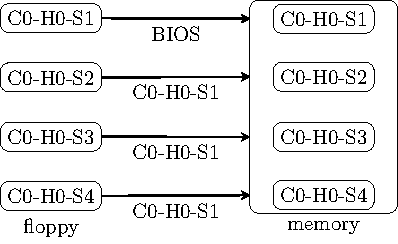
\includegraphics[width=.5\textwidth]{design.pdf}
  \todo[inline]{need a new figure}
  \caption{Workflow of the boot loader}
  \label{fig:working-flow-boot-loader}
\end{figure}

\missingfigure{MBR structure}

\todo[inline]{the 446 bytes code in MBR is for \ldots}

The instructions of the boot loader saved in C0-H0-S1 of floppy, the first cylinder, head 0,
the first sector, total 512 byte. These instructions end with \texttt{0x55 0xaa}, so BIOS will load
C0-H0-S1 to memory, then the instructions in C0-H0-S1 will load C0-H0-S2 --- C9-H1-S18,
total $10*2*18*512=184320byte=180KB$(including boot sector, C0-H0-S1) to main memory.

\subsection{32-bit Mode and Import C Codes}
\label{sec:32-bit-mode}


\chapter{Implementation}

\section{Boot Loader}

\subsection{Choose Disk}
\label{sec:chose-disk}

\todo[inline]{need rephrase}

There are many ways to boot an operating system, from hard disk, USB, floppy disk,
etc. \textcolor{red}{Among which, floppy disk is the simplest one to deal with, though
  it's out of date.} \xout{I choose floppy disk, although it is out of date.} \xout{For my
  purpose is that develop a simple operating system, pay my attention on how to
  development.} The structure of floppy disk is simple and for my simple operating system
it's enough.

\subsection{The Structure of a Floppy Disk}
\label{sec:struct-floppy-disk}

Fig.~\ref{fig:flpy1.png} shows the inside of a floppy disk:
\begin{figure}[!ht]
  \centering
  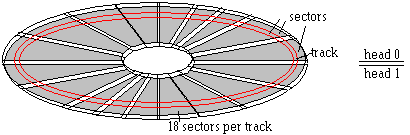
\includegraphics[width=.5\textwidth]{../figs/bootLoader/flpy1.png}
  \caption{Floppy Disk Structure}
  \label{fig:flpy1.png}
\end{figure}

A floppy disk\xout{, also called a floppy, diskette, or just disk,} is a type of disk
storage composed of a disk of thin and flexible magnetic storage medium, sealed in a
rectangular plastic enclosure lined with fabric that removes dust particles. Floppy disks
are read and written by a floppy disk drive (FDD)\verb|\cite{}|\todo{cite wikipedia}.

For $3.5$ inch HD floppy,  There are $80$ cylinders from the outermost to
the core on each side, numbering $0$, $1$, ..., $79$. The head can assign be $0$ or $1$,
representing two sides of floppy. When specify head number and cylinder number, forming a
ring, named track in jargon. The track is large so we divide it to 18 small parts, named
sector. A sector can store $512$ byte. So the capacity of a floppy is:

$$18 \times 80 \times 2 \times 512 = 1474560 Byte = 1440 KB$$

\subsection{Flowchart of Boot Loader}
\label{sec:flowch-boot-load}

Fig.~\ref{fig:flowchart-of-boot-loader} shows how the boot loader works.
\begin{figure}[!ht]
  \centering
  % 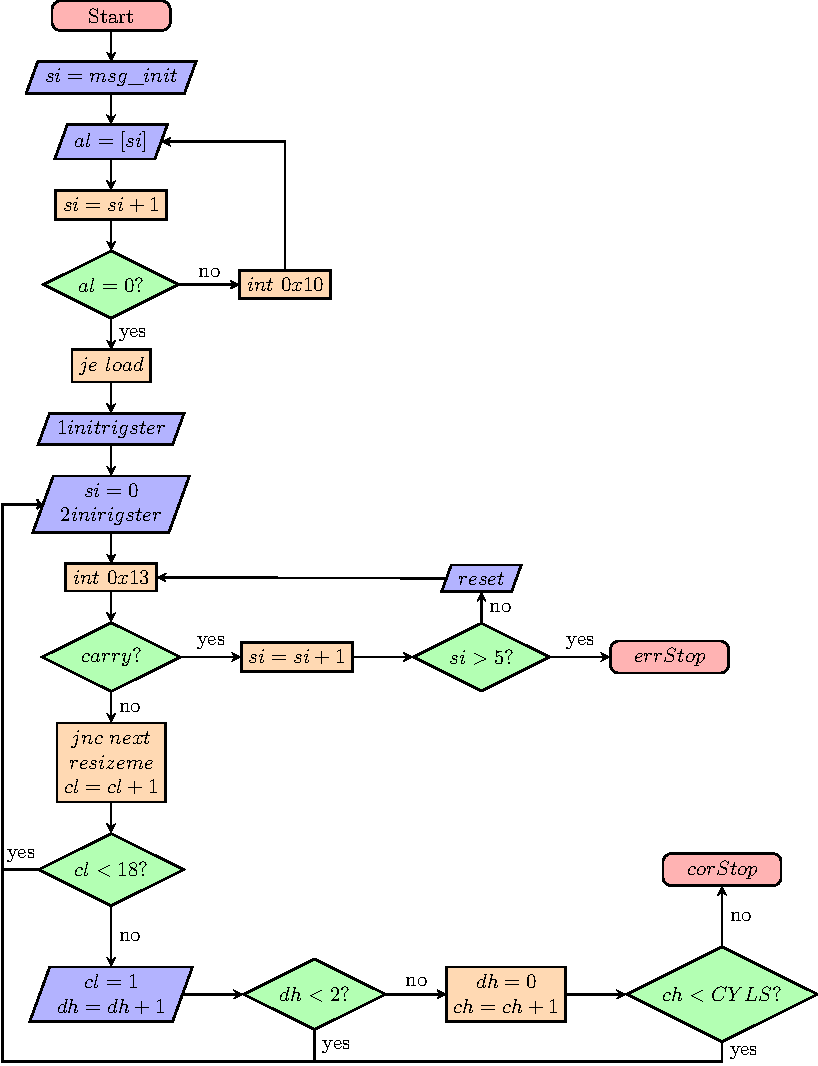
\includegraphics[width=1\textwidth]{../figs/FlowchartTex/1/flowcharte.pdf}
  \todo[inline]{need a better chart}
  \caption{Flowchart of Boot Loader}
  \label{fig:flowchart-of-boot-loader}
\end{figure}

The boot loader is implemented in Intel assembly. \textcolor{red}{It works as following:}

\begin{enumerate}
\item \textbf{Display boot information:} Firstly, the boot sector display some boot information,
  when $al=0$, the null character of boot information hit. Interrupt $0x10$ is used for
  show a character. Appendix ~\ref{sec:dis-boo-inf} is the code to perform this function.
\item \textbf{Read the second sector:} Then jump to load C0-H0-S2, $ax$ register saved the address
  where beginning puts the sectors from floppy. And preparing parameters for interrupt
  $0x13$ in registers. The $0x13$ interrupt used for read sector from floppy to
  memory. Appendix ~\ref{sec:rea-sec-sec} is the code to perform this function.
\item \textbf{Read two sides of a track:} If there is a carry, representing some thing wrong when
  read floppy, so reset the registers and try again read floppy, until five times
  trying. Register $si$ is a counter. If no carry, jump to next segmentation, as one
  sector read to memory already, the address space should increase 512 byte. Then sector
  number($cl$ register) added 1 and compare it to 18, if it's smaller than 18, jump to
  $readloop$, read the next sector. If the value of $cl$ register bigger or equal to than
  18, meaning that one track 18 sector in this side of floppy read already, then reversed
  the head, add 1 to $dh$ register. If the value of $dh$ register after adding larger than
  or equal to 2, it's saying the original head is 1, one track of two sides read
  already. Otherwise the value of $dh$ register smaller than 2, read this side indicating
  by $dh$ register, jump to $readloop$ segmentation. Appendix ~\ref{sec:rea-two-sid} is
  the code to perform this function.
\item \textbf{The next cylinder:} So the next step is moving a cylinder, add 1 to register
  $ch$. Otherwise the value of $dh$ register smaller than 2, read this side indicating by
  $dh$ register, jump to $readloop$ segmentation. After $ch$ register add 1, if it's
  smaller than 10, jump to $readloop$, otherwise end loading floppy to memory process, for
  we only load ten cylinders of floppy. Appendix ~\ref{sec:the-nex-cyl} is the code to
  perform this function.
\end{enumerate}

\subsection{Running Result}
\label{sec:running-result}

Fig.~\ref{fig:iplRes} shows the running results of boot loader. From this picture we
see that the boot loader loaded 10 cylinders from floppy successfully. 

\begin{figure}[!ht]
  \centering
  % 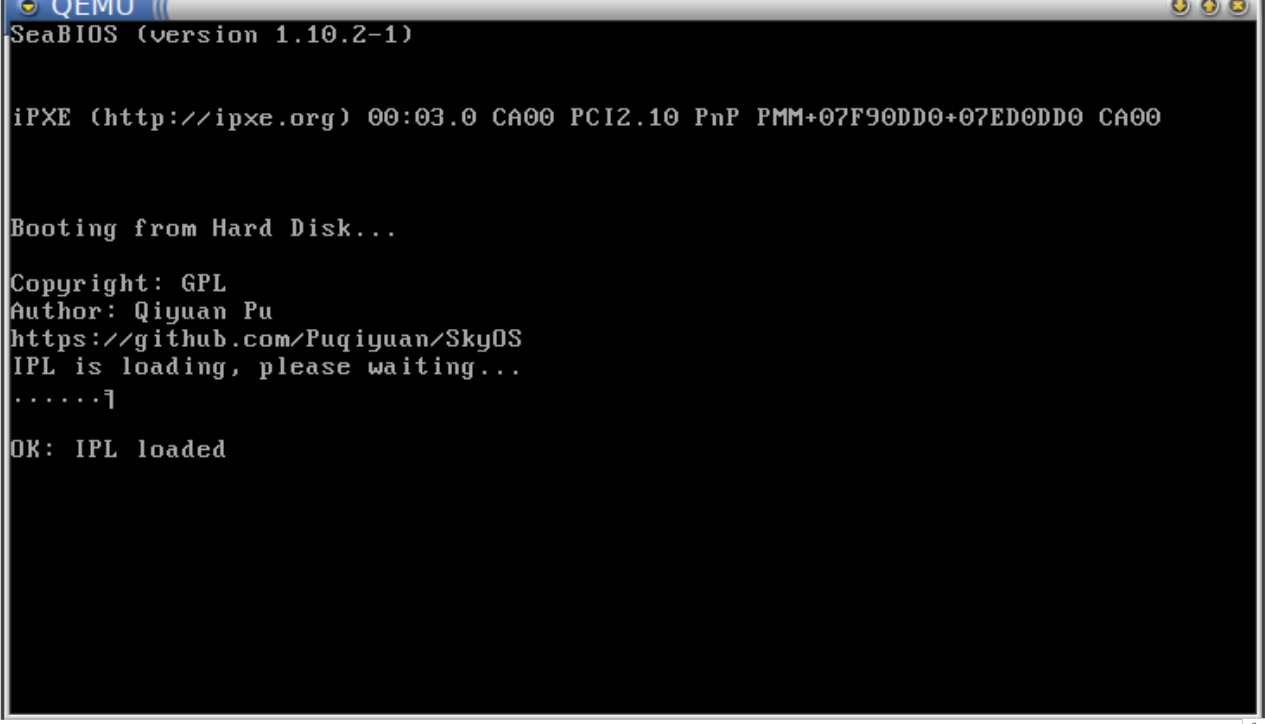
\includegraphics[width=1.1\textwidth]{iplRes.png}
  \todo[inline]{need a better pic.}
  \caption{Running Result of Boot Loader}
  \label{fig:iplRes}
\end{figure}



\section{32-bit Mode and Import C Codes}


\section{Screen Display and Text}

\section{Control Mouse}


\section{Memory Management}

\section{Making Window }

\section{Timer}

\section{Multitasking}

\section{Command Line Window}

\section{API}

\section{OS Protection}

\section{Graphics Processing}

\section{Window Operation}

\section{Application Protection}

\section{File Operation}

\section{Some Applications}

\chapter{Prospects And Shortages}

%%% 正文部分到此结束。下面是『参考文献』、『指导教师简介』、『鸣谢』、『附录』

%% 不要动下面四行!
\Appendix{}
\printbibliography[heading={bibintoc},title={参考文献}] % 输出参考文献
\advisorinfopage{}                 % 输出指导教师简介
\acknowledgmentspage{}             % 输出鸣谢

%%% 下面是附录部分,可以没有。

\chapter{Main Program Code} %附录一

\section{Boot loader}

\subsection{Display boot information}
\label{sec:dis-boo-inf}

\inputminted[firstline=55, lastline=65,
  linenos=true]{nasm}{../../src/06day/RongC/ipl10.nas}

\subsection{Read the second sector}
\label{sec:rea-sec-sec}
  
\inputminted[firstline=87,lastline=106,linenos=true]{nasm}{../../src/06day/RongC/ipl10.nas}

\subsection{Read two sides of a track}
\label{sec:rea-two-sid}

\inputminted[firstline=108,lastline=132,linenos=true]{nasm}{../../src/06day/RongC/ipl10.nas}

\subsection{The next cylinder}
\label{sec:the-nex-cyl}

\inputminted[firstline=134,lastline=137,linenos=true]{nasm}{../../src/06day/RongC/ipl10.nas}

\end{document} % 结束。不要动下面几行!

%%% Local Variables:
%%% mode: latex
%%% TeX-master: t
%%% End:
